%!TEX root = ../../dissertation.tex
%%%%%%%%%%%%%%%%%%%%%%%%%%%%%%%%%%%%%%%%%%%%%%%%%%%%%%%%%%%%%%%%%%%%%%%%%%%%%%%
\section{Modeling Mobile Network Load}
\label{c4:sec:modeling}

Drawing conclusions from statistical analysis alone is a difficult task. The next logical step lies therefore in the creation of models abstracting this real system, making them easier to calculate with the loss of some precision. This and future improved models should support network operators in predicting the signaling load in their core network with the benefit of improved network engineering and correctly scaling core components.


%%%%%%%%%%%%%%%%%%%%%%%%%%%%%%%%%%%%%%%%%%%%%%%%%%%%%%%%%%%%%%%%%%%%%%%%%%%%%%%
\subsection{Creating a Simple Toy Queuing Model}

\begin{figure}[htbp]
	\centering
	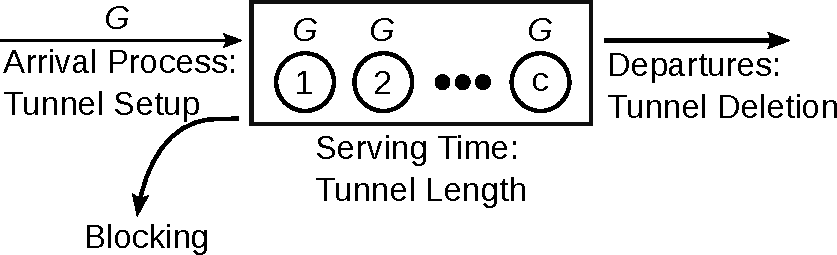
\includegraphics[width=\columnwidth]{images/GGn-model.pdf}
	\caption{Simple toy-model for tunnel-induced load on the core network.}
	\label{c4:fig:ggn-model}
\end{figure}

To begin the modeling process we attempt to represent the tunnel management as a queuing system, specifically as a G/G/n-0 system in Kendall's notation. Figure~\ref{c4:fig:ggn-model} shows this model for the case of our proposed tunnel load metric. Here, tunnels enter the system by a general random distribution, are then ``served'' at the \ac{GGSN} for the duration of their existence, which also follows a general distribution, and leave the system, i.e. are torn down, afterwards. If the serving units are filled, blocking occurs and arriving tunnel requests are rejected.

In this case ``servers'' correspond to available resources at one or more \ac{GGSN}, making the maximum number of tunnels hard to guess and depend on a number of factors. This could include soft-limits like the specific configuration, and hard-limits, e.g. the \ac{GGSN}'s processing and memory constraints. Unfortunately, all of these are unknown to us. Moreover, as the tunnels are all served on a relatively small number of hardware entities they are not independent of each other. Increasing load could very well influence both the arrival as well as the serving process.

For the purpose of creating a toy model we are further simplifying the G/G/n-0 to a M/M/$\infty$ queue. As stated, no actual limit to the number of virtual servers is known and the data also does not show any obvious limits. So we can safely assume an unlimited system and do not have to treat blocking or queuing explicitly.

\begin{figure}[htbp]
	\centering
	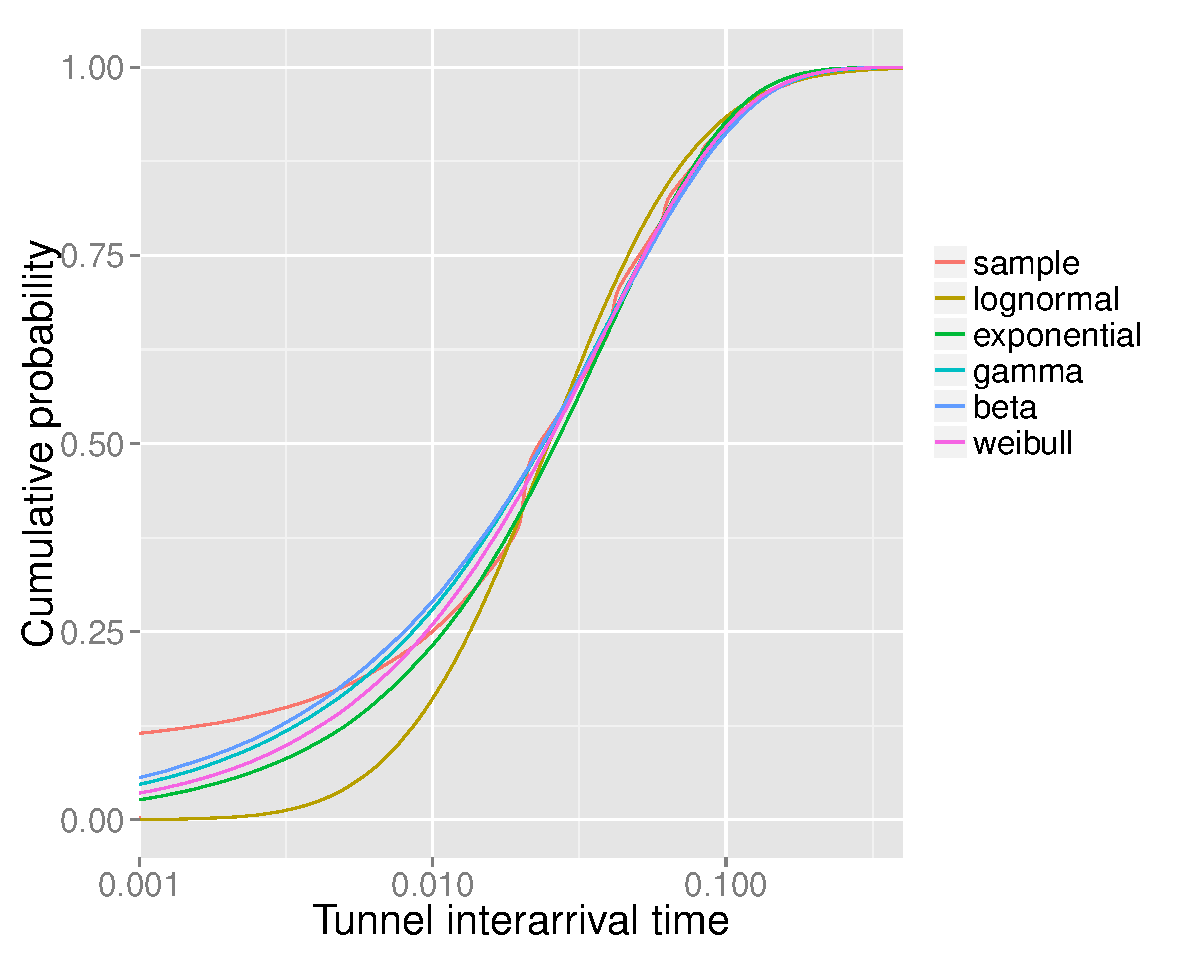
\includegraphics[width=\columnwidth]{images/R-IAT-ecdfs.pdf}
	\caption{Sampled inter-arrival time CDF and fitted theoretical distributions.}
	\label{c4:fig:IAT-cdfs}
\end{figure}

Furthermore, we fitted univariate distributions to the experimental data for the tunnel inter-arrivals and durations and tested the goodness of the fit both numerically, using Pearson's $\chi^2$ test, and visually for the density and CDF plots. No standard random distribution reaches the significance level for either process. We attribute this fact largely to the various artifacts in the data, e.g. the described wave effect every 20 milliseconds in the inter-arrival time. Matching them visually (confer also the cumulative distribution function plot in Figure~\ref{c4:fig:IAT-cdfs}) we find that the exponential fit is reasonably close to the experimental data in both the arrival and duration cases. Again, these distribution fits are just for a toy model to lay the groundwork for future and improved modeling.


\begin{figure}[htbp]
	\centering
	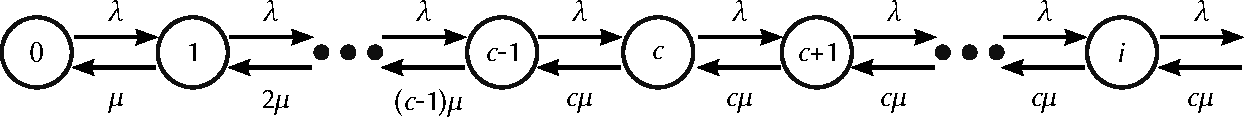
\includegraphics[width=\columnwidth]{images/markovchain.pdf}
	\caption{Markov chain model for the tunnel serving process.}
	\label{c4:fig:markovchain}
\end{figure}

Now, assuming both a Poisson arrival and an exponential serving process, a Markov chain representing the queue can be set up (cf. Fig.~\ref{c4:fig:markovchain}) and stationary analysis can be conducted. From the measured data an arrival rate of $\lambda=25.64123$ and the parameter $\mu=0.0001586728$ for the exponential service time distribution are calculated. Using Little's Law this gives an estimate for the mean number of concurrent tunnels at the \ac{GGSN} of 

$$
L=\frac{\lambda}{\mu}\approx 161\,599. %=161598.14.
$$

As stated, the amount of state held at the node and propagated through the network is directly related to the number of tunnels. Therefore, we propose this metric as an initial estimate of the load at the \ac{GGSN}.


%%%%%%%%%%%%%%%%%%%%%%%%%%%%%%%%%%%%%%%%%%%%%%%%%%%%%%%%%%%%%%%%%%%%%%%%%%%%%%%
\subsection{Advanced Models} 



%%%%%%%%%%%%%%%%%%%%%%%%%%%%%%%%%%%%%%%%%%%%%%%%%%%%%%%%%%%%%%%%%%%%%%%%%%%%%%%
\subsection{Simulative Validation} 



%%%%%%%%%%%%%%%%%%%%%%%%%%%%%%%%%%%%%%%%%%%%%%%%%%%%%%%%%%%%%%%%%%%%%%%%%%%%%%%
\subsection{Modeling Discussion}

On the basis of this toy model better fitting models can now be constructed. Those should also factor in more of the core network's properties and specified parameters omitted in this model. Specifically, this means shifting from M/M/$\infty$ to the more generalized G/G/n and therefore finding better distribution fits for the involved processes.

It is also entirely possible that the single queue approach is not the best way to describe control plane load. Several load influencing factors discussed earlier have direct influence on the tunnel arrivals and duration, e.g. the device type or the radio access technology. Therefore, amongst others multidimensional queuing networks or fluid flow could be a better fit. Our plan is to conduct further investigations into the modeling of mobile core network signaling. This also includes a rough simulative approach, which could also be used to validate our models against experimental data.

